\documentclass[main.tex]{subfiles}
\begin{document}

\section{Digitized Waveform Neutron Tagging}

\subsection{Energy Calibrated QDC spectrum}
The raw pulses are integrated over 500 ns starting 10 ns before the peak of the pulse. This yields the uncalibrated QDC spectrum. In order to calibrate the spectrum to electron equivalent energy the compton edges of the PuBe source as well as a $^{60}Co$ source were used. The energy calibration was performed with the Knox method as was the case for the analog setup. The 2.23 and 4.44 $MeV_{ee}$ compton edges are marked in green and red respectively in the top plot in fig \ref{fig:D_QDC}. The $^{60}Co$ source has compton edges at 1.17 and 1.33 $MeV_{ee}$, but they can not be distinguished. Instead they are treated as a single peak located at their midpoint at 1.25 $MeV_{ee}$. 

As fig \ref{fig:D_QDC} shows points fit neatly on a stright line. The fit parameters are used to produce tghe calibrated energy spectrum shown below.

The surprising peak near 12 $MeV_{ee}$ is due to events thatwere cut off by the range of the digitizer. These are likely cosmic muons.
\begin{figure}[ht]
    \centering
        \includegraphics{DigitalResults/Ecall.pdf}
        \caption{The 1.17 + 1.25 MeV edge of the $^60$ source and the 2.23 and 4.44 MeV Compton edges of the PuBe source have here been used to perform an energy calibration. Due to the event by event based baseline determination it is assumed that bin 0 corresponds to 0 $MeV_{ee}$}
    \label{fig:D_QDC}
\end{figure}



\subsection{Pulse shape discrimination}
\subsubsection{Charge comparisson method}
The pulses were also integrated over a 60 ns window in order to compare the fraction of deposited energy in the pulses tail to the total deposited energy. The result is shown in fig \ref{fig:psd_d}. As with the analog setup longgate and shortgate offsets can be used to linearize the seperation between the bands. Here a shortgate offset 25 mV and a longate offset offset of 3 mV were used to linearize the seperation between neutron and gamma bands. Below 1.5 $MeV_{ee}$ the bands start starts to mix considerably.

The 1.23 $MeV_{ee}$ and 4.44 $MeV_{ee}$ compton edges are clearly distinguishable in the lower band. The neutrons have a continuous energy distribtion and as such we don't see any sharp peaks in their band. 

\begin{figure}[ht]
    \centering
        \includegraphics{DigitalResults/psd.pdf}
        \caption{Pulse shape discrimination spectrum produced with the charge comparisson method.}
        \label{fig:psd_d}
\end{figure}

\subsubsection{Convolutional neural network based discrimination}
The convolutional neural network described in \ref{sec:cnn} was applied to the data presented in this chapter. Since the activation function of the output node is the logistic function the value is bounded between zero and 1. The resulting pulse shape discrimination spectrum is shown in fig \ref{fig:cnn_E} as a function of deposited energy. Like for the charge comparisson method the upper distribution is neutrons and the lower distribution consists of gammas, and again the 2.23 and 4.44 $MeV_{ee}$ are clearly visible in the gamma band. Furthermore most of the low energy pulses have been identified as gammas.


\begin{figure}[ht]
    \centering
        \includegraphics{DigitalResults/CNNpsd.pdf}
        \caption{Pulse shape discrimination spectrum produced with a convolutional neural network.}
    \label{fig:cnn_E} 
\end{figure}

\clearpage
\subsection{Time of flight spectrum}
The time of flight spectrum acquired in 1 hour of data taking is shown in fig \ref{fig:D_TOF}. The gamma peak is centered at 3.3 ns and the neutron distribution stretches from around 35 to 65 ns. The gamma peak is not entirely narrow as one might expect seeing as they all travel at the speed of light. As for the analog setup part of the reason is that each photon may have a longer or shorter flightpath depending on its point of production in the source and the point at which it interacts in the detector. How far they travel in the detector mdium will also vary. There is also some uncertainty due to the active splitter as well as the digitization. On top of that the timestamp of each event is limited by the sampling rate of the digitizer. Although the cfd trigger algorithm interpolates between neighbouring points it still relies on the peak amplitude, whose precision is limited by the digitizers sampling rate.
\begin{figure}[ht]
begin{figure}
    \centering
        \includegraphics{DigitalResults/tof.pdf}
        \caption{The time of flight spectrum of the PuBe source produced by the digital setup.}
    \label{fig:D_TOF} 
\end{figure}

Plotting pulse shape discrimination parameters against time of flight can be used to confirm that we are indeed seperating gamma and neutrons with the PSD algorithms. This is shown in figure \ref{fig:tof_cc_tof_cnn}. In fig \ref{fig:tof_digi_cc} we see the narrow gamma distribution and the wider neutron distribution. It is apparent that the two distributons overlap. In fig \ref{fig:tof_digi_cc} the distribution are better separated, but it still appears that gammas and neutrons overlap slightly near prediction value 0.5.
\begin{figure}
    \centering
    \begin{subfigure}[ht]{\textwidth}
        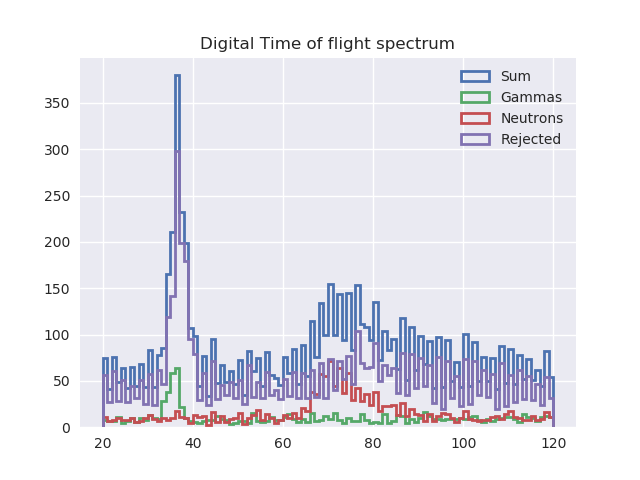
\includegraphics{DigitalResults/tof_psd.pdf}
        \caption{}
        \label{fig:tof_digi_cc}
    \end{subfigure}
	\begin{subfigure}[ht]{\textwidth}
        \includegraphics{DigitalResults/CNNtof_psd.pdf}
        \caption{}
        \label{fig:tof_digi_cnn}
    \end{subfigure}
    \caption{heatmaps of of pulseshape discrimination parameters as functions of time of flight plotted with logarithmic z-axis.}
    \label{fig:tof_cc_tof_cnn}
\end{figure}

A perfect PSD algorithm (assuming only neutrons and gammas interact in the detector) would be able to filter the time of flight spectrum into a pure neutron spectrum and a pure gamma spectrum. fig \ref{fig:tof_filt_cc} shows the resulting time of flight spectrum when a cut is made at tail/total = 0.141. The neutron distibution is not flat at the gamma peak and the gamma distribution is not flat at the neutron distrubution, so there is clearly some misclassification happening. As was seen in \ref{fig:psd_d} This is mostly due to the neutron and gamma bands overlapping significantly at deposited energies below 2 $MeV_{ee}$.





\end{document}